%%%%%%%%%%%%%%%%%%%%%%%%%%%%%%%%%%%%%%%%%%%%%%%%%%%%%%%%%%%%%%%%%%%%%%%%
\chapter{Vergleich}
\label{sec:comparison}
%%%%%%%%%%%%%%%%%%%%%%%%%%%%%%%%%%%%%%%%%%%%%%%%%%%%%%%%%%%%%%%%%%%%%%%%
Es folgt nun eine Gegenüberstellung der einzelnen Frameworks, anhand der in Kapitel \ref{sec:methodik} definierten Kriterien. Als erster wird ein genereller Überblick über die einzelnen Fakten zu den Frameworks gegeben und deren Unterschiede hervorgehoben. Danach wird noch genauer auf relevanten Kriterien für das Revex Projekt eingegangen.

\section{Gegenüberstellung der Frameworks}

\textbf{Performance}\\
Mobile Geräte haben längst Einzug in das Alltagsleben erhalten, viele Nutzer erweitern die Funktionalität der Geräte mit zahlreichen Anwendungen. Jede installierte App auf einen mobilen Endgerät hat Einfluss auf den Energieverbrauch. Je mehr Anwendungen auf eine Endgerät installiert sind und je öfter diese genutzt werden, desto höher ist der Energieverbrauch und die Betriebszeit sinkt dadurch massiv \cite{Wil2012}. Daher ist bei der Entwicklung darauf zu achten, das der Energieverbrauch so gering wie möglich gehalten wird. Auswirkungen auf den Energieverbrauch eines Smartphones haben sowohl der Bildschirm, die \acrfull{CPU}, die Kommunikation über das Mobilfunknetz, als auch das WLAN-Modul. Werden die einzelnen Komponenten so wenig wie möglich beansprucht, ist der Energieverbrauch der Anwendung gering \cite{vetter}. 
\\\\
Umso länger und mehr Daten bei einem Request über das Mobilfunknetz oder das WLAN-Modul übertragen werden, desto mehr Energie wird verbraucht. Es sollte daher darauf geachtet werden, dass die Requestdauer möglichst gering ist und nicht unnötige Daten übertragen werden. Des weiteren ist die Rechenleistung von Smartphones  wesentlich geringer als jene von Notebooks, um die Betriebszeit zu erhöhen. Daher ist bei der Entwicklung auch darauf zu achten, dass die CPU Beanspruchung der Apps gering gehalten wird, damit das System performant weiterarbeiten kann \cite{mittal:energy}. Außerdem sollte die benötigte CPU Leistung aus einem weiteren Grund möglichst gering sein, den die Hardware variiert von Smartphone zu Smartphone. Ist die benötigte CPU Leistung gering, ist es möglich die App auf nahezu allen mobilen Geräten zu installieren und zu starten \cite{joorabchi:challenges}. 
\\\\
Für den Performance Vergleich wurden daher sowohl die CPU-Auslastung, als auch die Dauer für GET- und POST Requests (Dauer der Netzwerkkommunikation) der einzelnen Frameworks gegenübergestellt. Um Vergleichswerte zu ermitteln, wurden jede App einzeln in einem Emulator gestartet und die gleich Abfolge an Funktionsaufrufen durchgeführt. 
\\\\
Die Zeitdauer der GET-Requests bei der Abbildung \ref{getRequests} setzt sich aus 11 einzeln abgesetzte GET-Requests zusammen. Diese Requests werden benötigt, um die Details zu einem bestimmten Kraftwerke anzuzeigen. Es werden in der Praxis oft mehrere GET-Request hintereinander abgesetzt, daher wurde die Dauer ermittelt um alle Details zu einem Kraftwerk abzurufen. Es konnte dabei festgestellt werden, dass Retrofit am schnellsten ist, dicht gefolgt von AndroidAnnotations und Jersey am langsamsten ist.
\newpage

\begin{figure} [ht]
	\centering
	\subfloat[GET Request Retrofit]{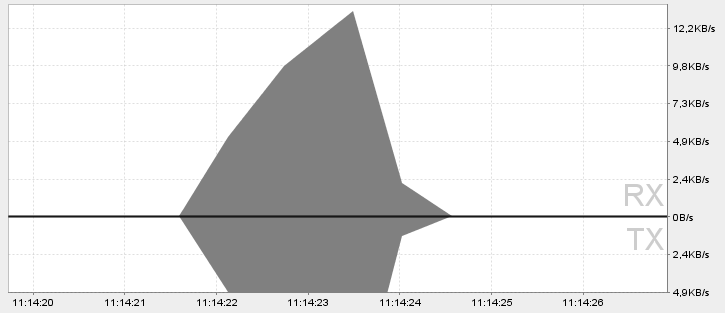
\includegraphics[width=0.45\textwidth]{figures/get_retrofit.png}} \qquad
	\subfloat[GET Request Jersey]{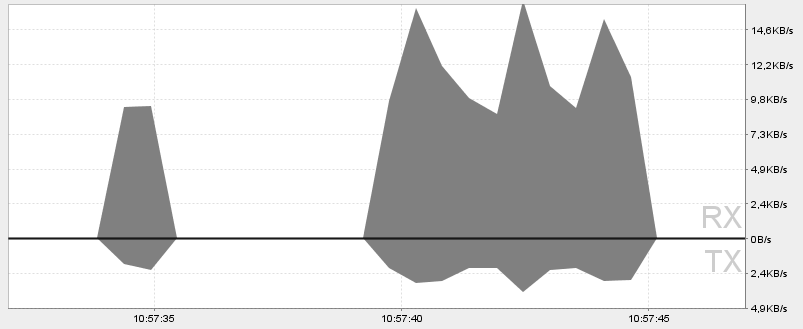
\includegraphics[width=0.45\textwidth]{figures/get_jersey.png}} \qquad
	\subfloat[GET Request Spring for Android]{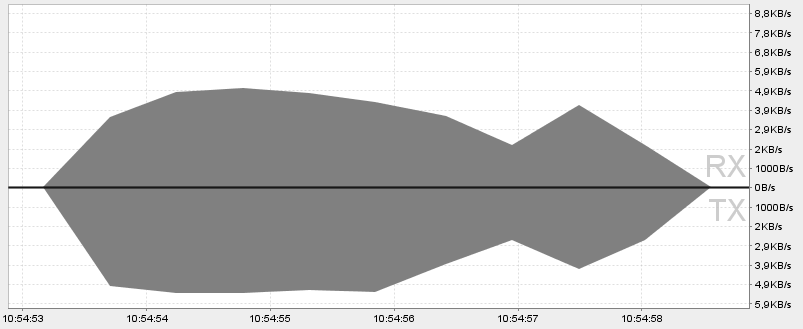
\includegraphics[width=0.45\textwidth]{figures/get_spring.png}} \qquad
	\subfloat[GET Request AndroidAnnotations]{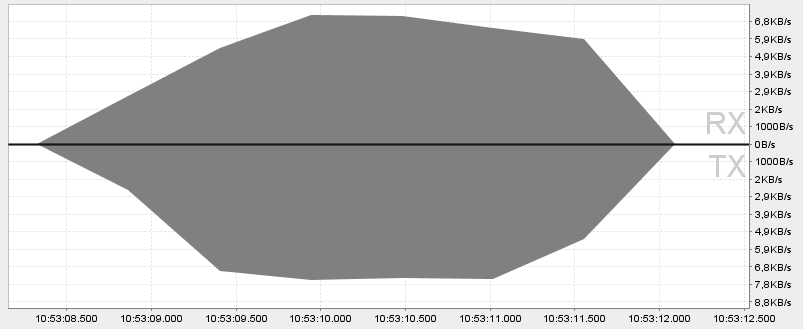
\includegraphics[width=0.45\textwidth]{figures/get_aa.png}}
	\caption{Zeitmessung der GET Requests} 
	\label{getRequests}
\end{figure} 

Die Messung der Zeitdauer für einen POST Request ist aus der Abbildung \ref{postRequests} zu entnehmen. Dabei wurde die Zeit gemessen, bis neu eingegeben Daten um ein neues Kraftwerk anzulegen, erfolgreich zum Server übermittelt wurden. Es konnte dabei festgestellt werden, dass alle Frameworks circa gleich lange benötigen, um die Daten zu übertragen. Spring for Android ist dabei minimal langsamer als die anderen, dies ist aber zu vernachlässigen, da diese Verzögerung keine Auswirkung auf die Usability für einen User hat \cite{meyer:performance}.

\begin{figure} [ht]
	\centering
	\subfloat[POST Request Retrofit]{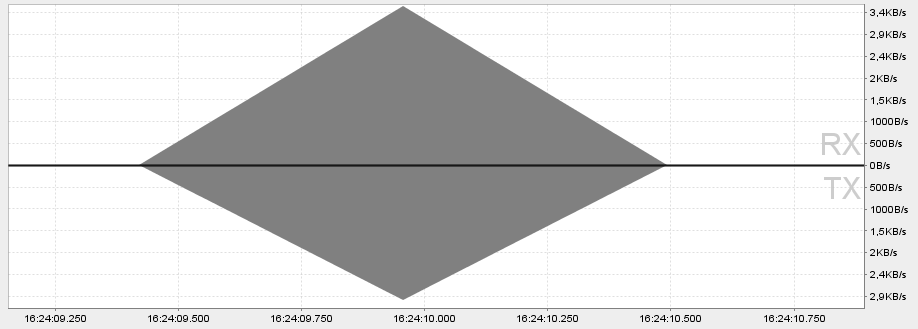
\includegraphics[width=0.45\textwidth]{figures/post_retrofit.png}} \qquad
	\subfloat[POST Request Jersey]{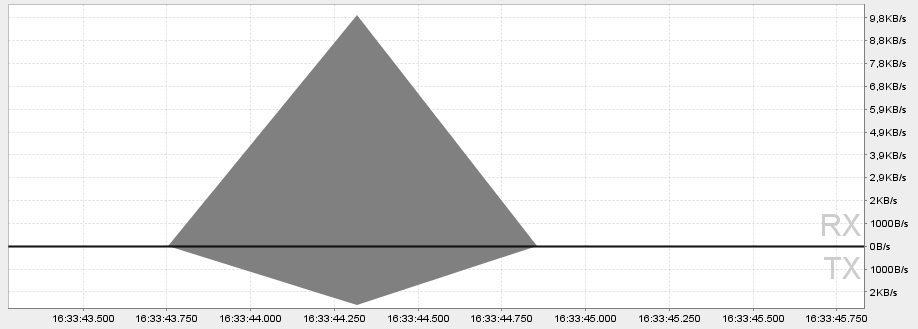
\includegraphics[width=0.45\textwidth]{figures/post_jersey.png}} \qquad
	\subfloat[POST Request Spring for Android]{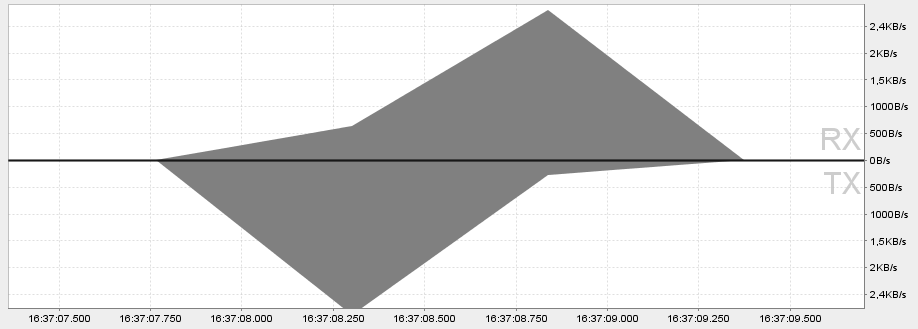
\includegraphics[width=0.45\textwidth]{figures/post_spring.png}} \qquad
	\subfloat[POST Request AndroidAnnotations]{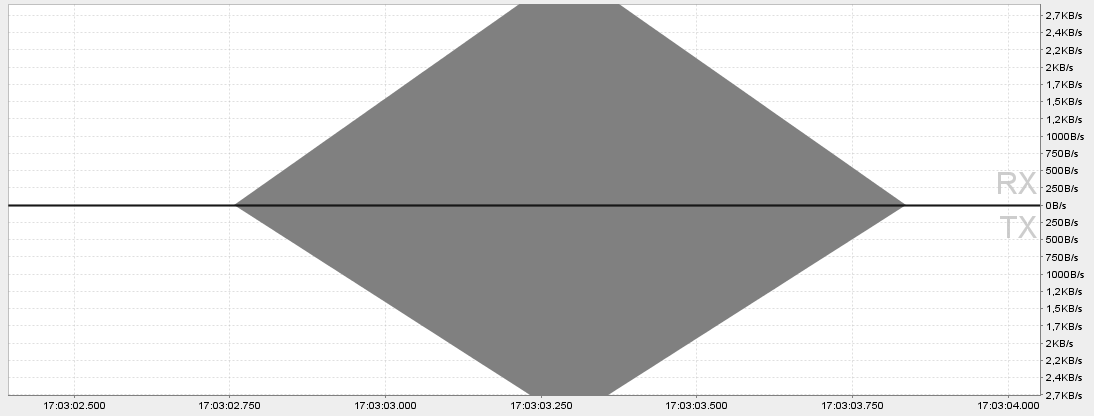
\includegraphics[width=0.45\textwidth]{figures/post_aa.png}}
	\caption{Zeitmessung der POST Requests} 
	\label{postRequests}
\end{figure} 

In der Abbildung \ref{cpuAuslastung} wird die CPU Auslastung der einzelnen Frameworks gegenübergestellt. Aus dieses Abbildung kann entnommen werden, das AndroidAnnotations die CPU am geringsten in Anspruch nimmt und Jersey am stärksten. Bei der Benutzung der Apps ist auch festzustellen, dass AndroidAnnotations und Retrofit am schnellsten arbeiten und eine flüssige Bedienung der Anwendung möglich ist. Jersey ist des öfteren langsam und hat kleine Ruckler währende der Bedienung.  

\begin{figure} [ht]
	\centering
	\subfloat[CPU Auslastung Retrofit]{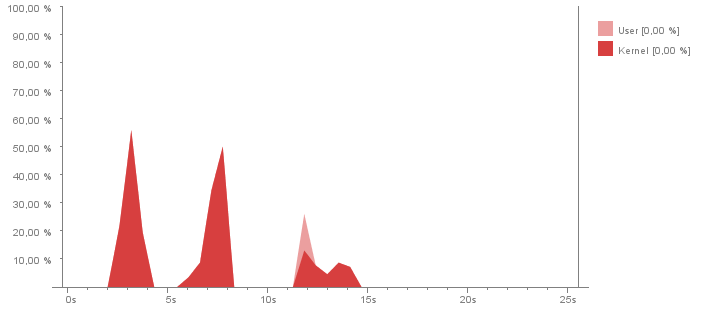
\includegraphics[width=0.45\textwidth]{figures/cpu_retrofit.png}} \qquad
	\subfloat[CPU Auslastung Jersey]{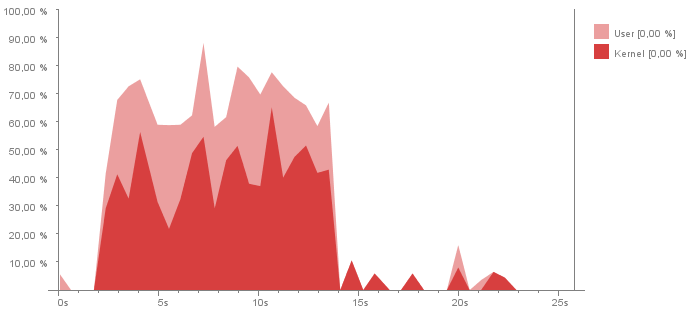
\includegraphics[width=0.45\textwidth]{figures/cpu_jersey.png}} \qquad
	\subfloat[CPU Auslastung Spring for Android]{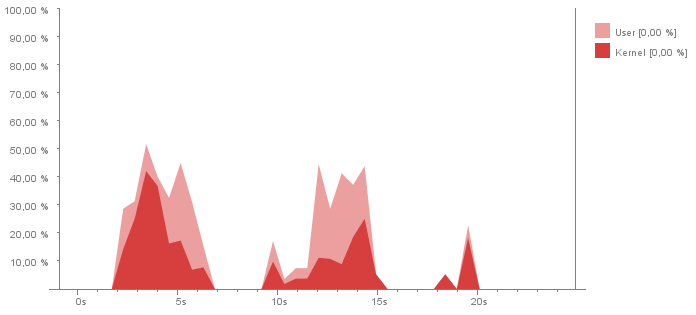
\includegraphics[width=0.45\textwidth]{figures/cpu_spring.png}} \qquad
	\subfloat[CPU Auslastung Request AndroidAnnotations]{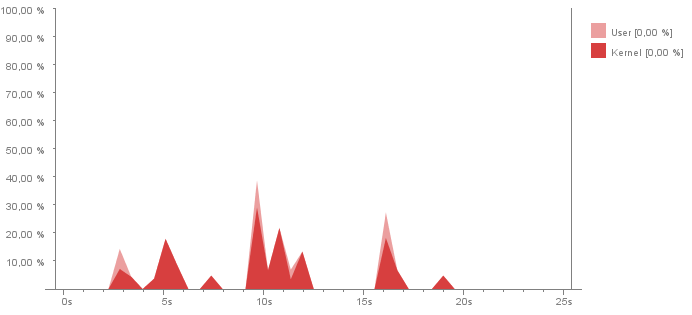
\includegraphics[width=0.45\textwidth]{figures/cpu_aa.png}}
	\caption{CPU Auslastung} 
	\label{cpuAuslastung}
\end{figure} 

\newpage
\textbf{Speicherplatz}\\

\begin{landscape}
	
\begin{tabular}{p{3.2cm}|p{4.8cm}|p{4.8cm}|p{4.8cm}|p{4.8cm}}
   & \textbf{Retrofit} & \textbf{Jersey} & \textbf{Spring for Android}  & \textbf{AndroidAnnotations}  \\  \hline
  \textbf{Lizenz} &
  Apache License 2.0 & 
  CDDL und GPL 2.0 & 
  Apache License 2.0 & 
  Apache License 2.0 und CDDL \\ \hline
  \textbf{Community} \\ \hline
  \textbf{Dokumentation} \\ \hline
  \multicolumn{5}{c}{\textbf{Performance}} \\ \hline
  
  \textbf{Zeit GET Request} & \textasciitilde3s & \textasciitilde12s  & \textasciitilde5s & \textasciitilde3.5s\\ \hline
  
  \textbf{Zeit POST Request} & \textasciitilde1s &  \textasciitilde1s & \textasciitilde1.5s & \textasciitilde1s \\ \hline
  
  \textbf{CPU Auslastung} & max. \textasciitilde55\%  & max. \textasciitilde87\% & max. \textasciitilde52\% & max. \textasciitilde40\%\\ \hline
\end{tabular} 

Heap Size:
AA: 6,469 MB	
Jersey: 10.913 MB
Spring: 8,546 MB
Retrofit: 6,727 MB

\end{landscape}

\section{Persönliches Fazit zu den Frameworks}

\textbf{Jersey}
\\\\
\textbf{Retrofit}
\\\\
\textbf{Spring for Android}
\\\\
\textbf{AndroidAnnotations}
\\\\